\label{ch:appendix_ABM}

\newpage
\subsection{ABM}

\begin{figure} [H] %plot-design
\centering
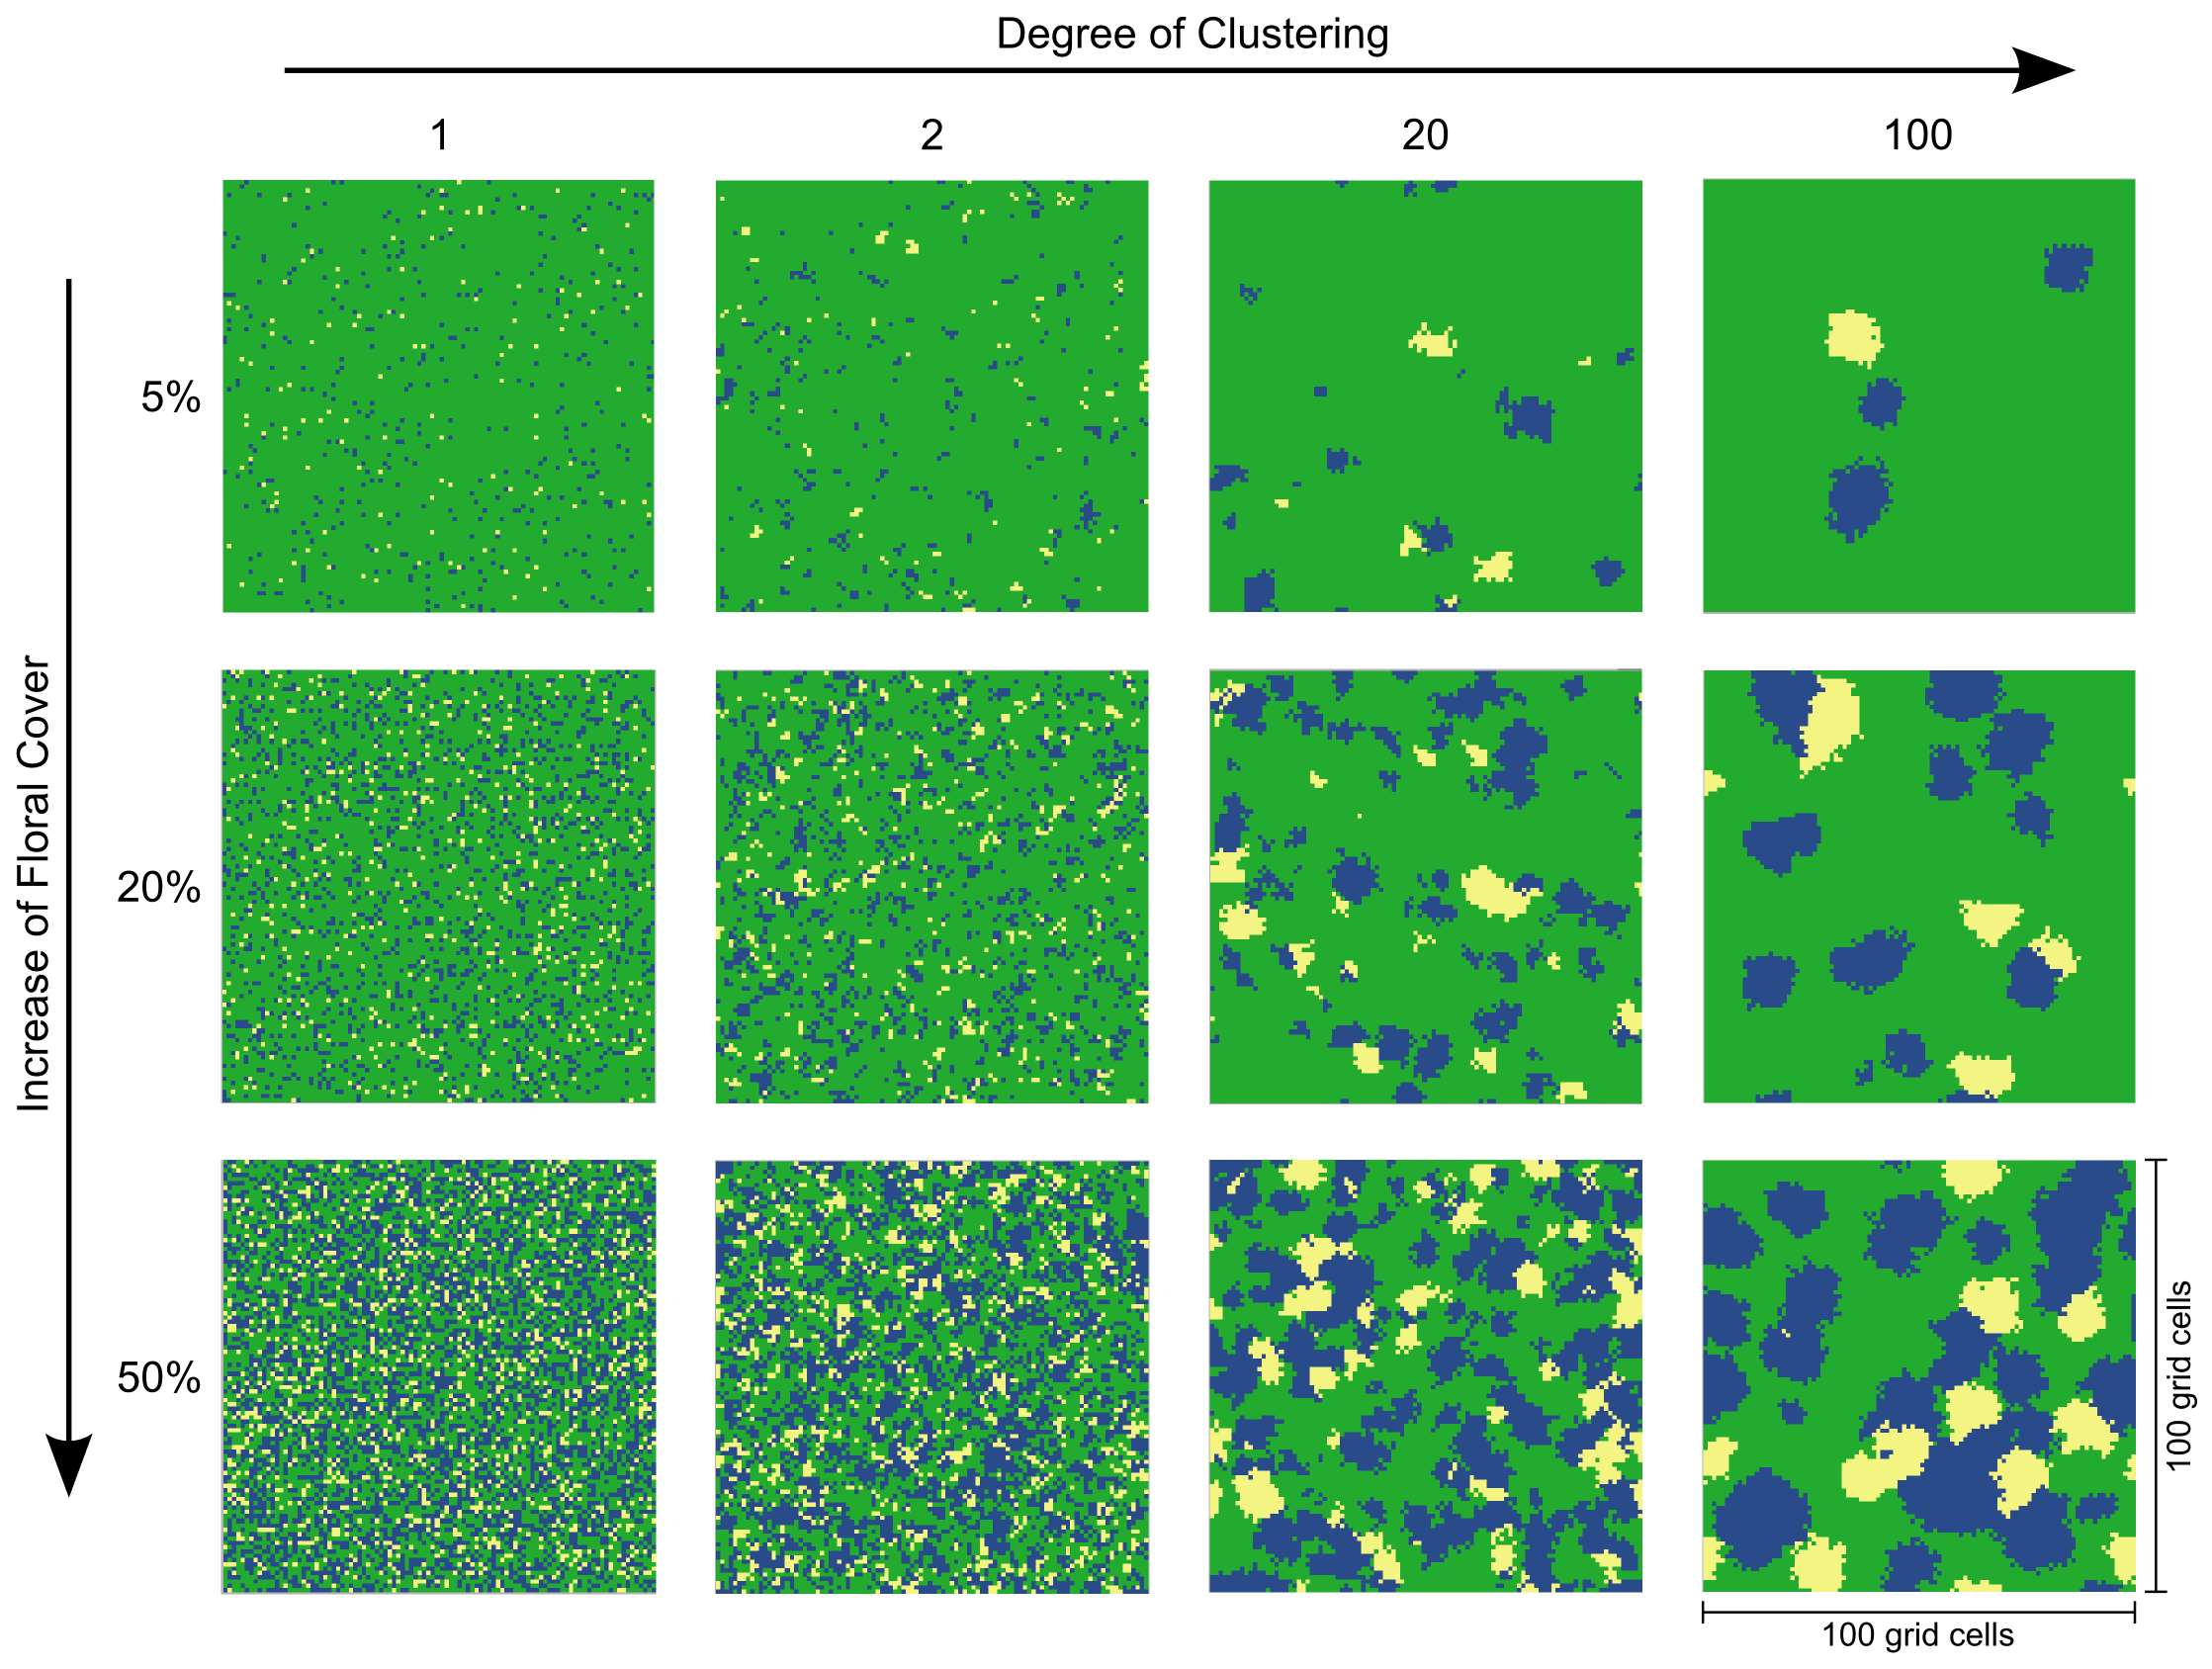
\includegraphics[width=15cm]{Images/cluster}
 \caption{ Exemplary model environment setups with increasing floral cover and degree of clustering. The cover expresses the percentage of patches containing a flower ($\Sigma_{patches}$ = 10 000). The cluster number equals the average amount of flowers per cluster. Flowers are randomly assigned to the clusters to achieve a more natural, uneven distribution. }
 \label{fig:cluster}
\end{figure}

%%%%%%%%%%%%%%%%%%%%%%%%%%
\newpage


\begin{figure} [H] %flowchart
\centering
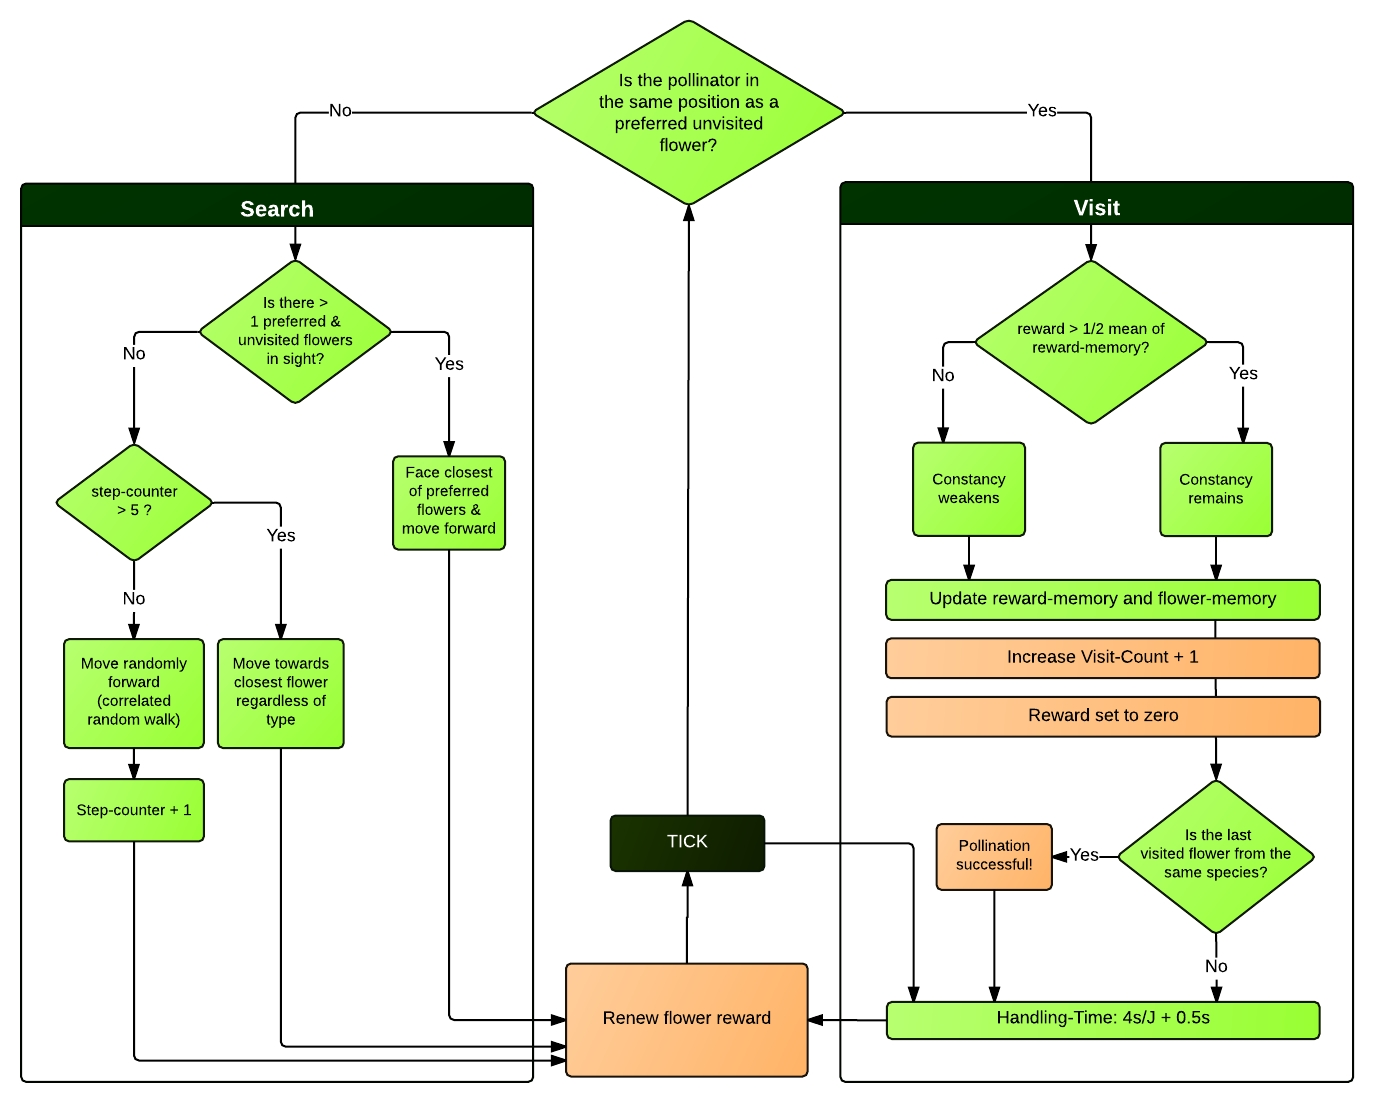
\includegraphics[width=15cm]{Images/flowchart-model}
 \caption{Flowchart describing the behavior rules for the bee-agents within the agent-based model. Every bee-agent can either search for a preferred flower or visit one. While searching, a bee-agent can remember the location of the last four visited flowers to avoid double-encountering. If there is no flower in sight after 5 seconds of correlated random walk (CRW), the probability that it will encounter the next available flower despite its type increases by 10\% per additional time step. When a bee-agent visits a flower it takes all reward within a reward-dependent handling time and compares the amount with its memory. If the reward is low, the agent is more likely to visit the other flower type next time. The maximum of visits within a successful pollination is possible is determined by the pollen carryover rate.}
 \label{fig:flowchart}
\end{figure}


%%%%%%%%%%%%%%%%%%%%%%%%%%
\newpage

\begin{table} [!htbp]
 \centering
  \caption{Parameter values used for the main and sensitivity analysis. Only general parameters were changed in the main analysis, whereas the sensitivity analysis also influenced the behavior of the bee-agents. Within the main analysis, Each combination was run 20 times for 1000 ticks (total of 110400 simulation runs) }
   \begin{tabular} {l l l}
    \toprule
    \textbf{Parameter} & \textbf{Description}  & \textbf{Values}\\
   \midrule
   \addlinespace[0.2cm]
   \multicolumn{ 3} {l} {\textsc{Main analysis}} \\ 
   \addlinespace[0.2cm]
Frequency & Proportion of species A on all flowers  & 0-100\% (5\%-steps)\\
Flower cover & Proportion of patches being flowers  & 5, 10, 20, 50 \%\\
Degree of clustering & Average number of flowers per cluster   &  1, 2, 5, 10, 20, 50, 75, 100\\
Pollen-carryover rate & Number of visits within a successful pollination is possible & 1, 2, 4, 6, 8, 16\\

\addlinespace[0.2cm]
\multicolumn{ 3 } {l} {\textsc{Sensitivity analysis}} \\ 
\addlinespace[0.2cm]
Reward function & Increase of reward per flower and second & 0, 0.00004, 0.001, 0.1 J/sec \\
Vision distance & Maximum range of patches within a bee-agent can detect flowers & 1, 6, 20, 50 patches\\
Search time & \begin{tabular}{@{}l@{}} Number of seconds a bee-agent searches before\\ probability of switching flowers increases \end{tabular}   & 1, 5, 20, 50 sec \\
Pollinator density & Number of bee-agents on the meadow & 5, 10, 20, 50 bees\\

    \bottomrule
    \end{tabular}
    \label{tab:simulation_run}
\end{table}


%%%%%%%%%%%%%%%%%%%%%%%%%%
\newpage


\begin{figure} [!h]
	\centering
	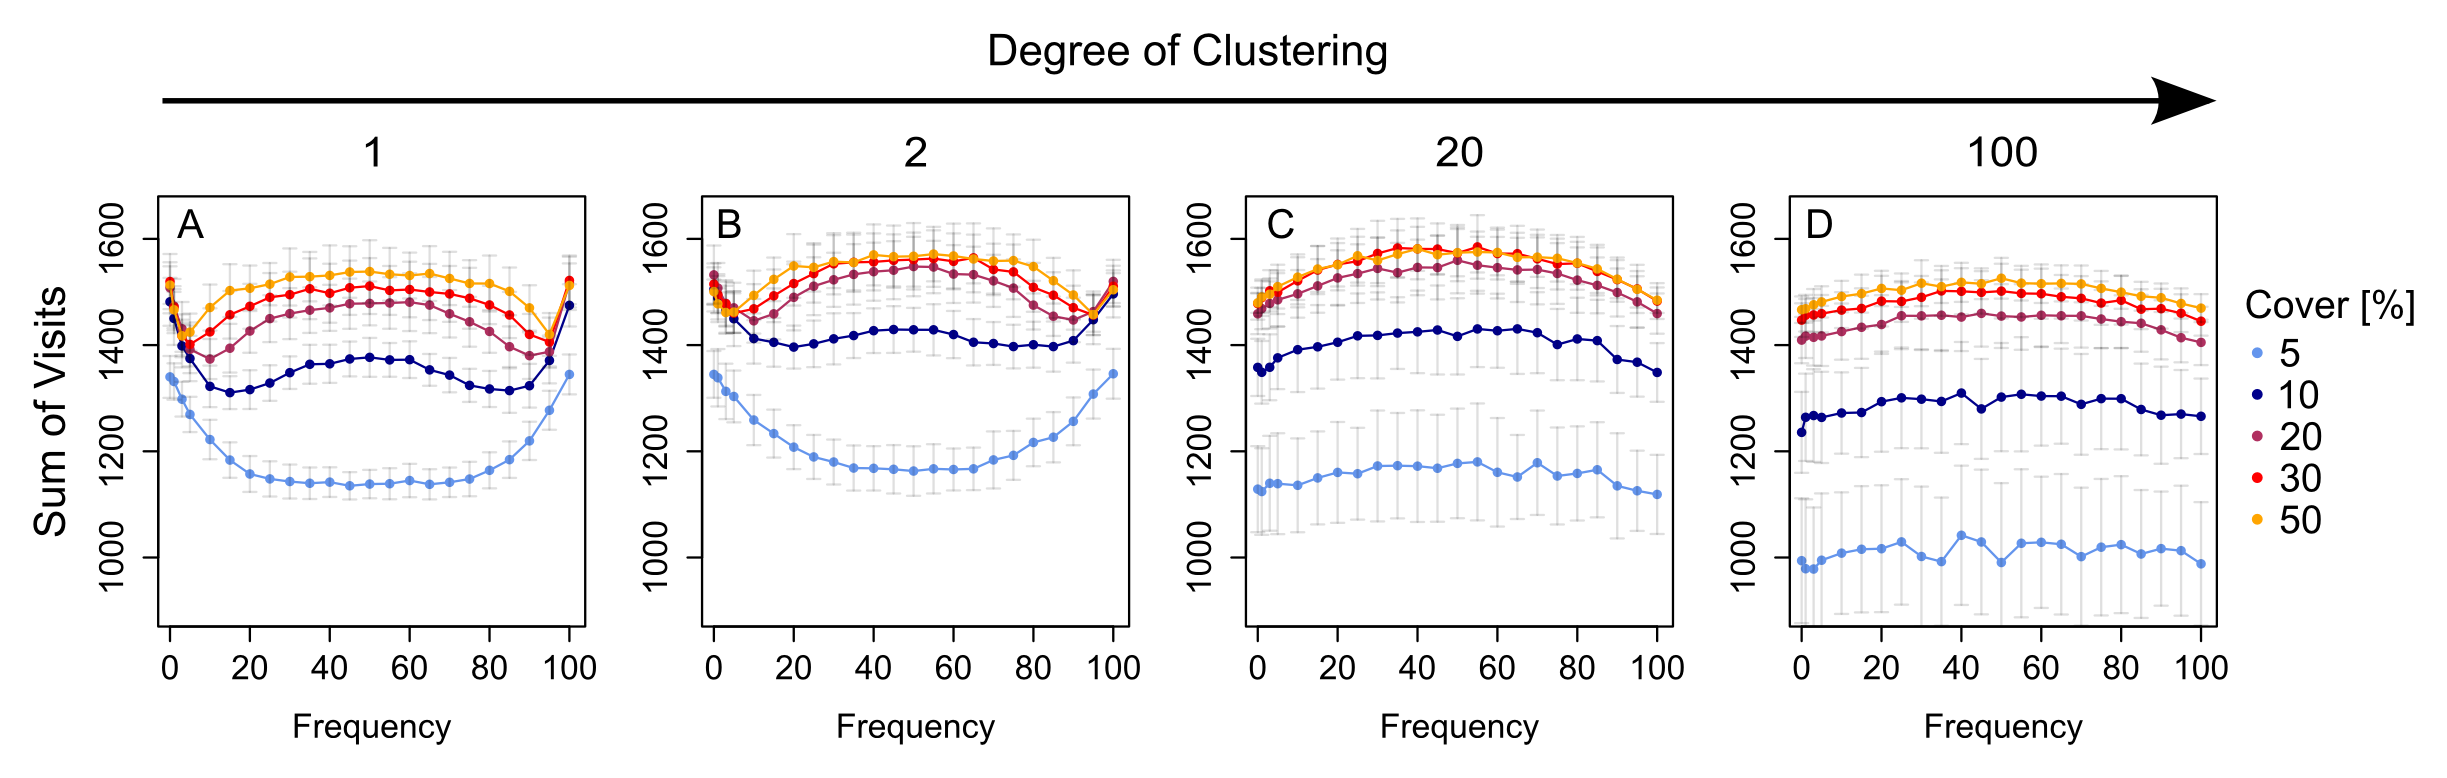
\includegraphics[width=17cm]{Images/SUM}
	\caption{Summed visits to both species show a frequency dependence for low cluster values. Depending on the floral cover it is quadratic or a fourth-degree polynomial relationship. Maximum of visits (maximal efficiency) is achieved for very unequal or very equal frequencies. If one species is rare, the sum of visits drop because some bee-agents forage inefficiently on the rare species, having long flight and searching times. Clustering reduces the frequency dependence but also decreases the absolute number of visits and increases the variance (grey error bars).}
	\label{fig:SUM}
\end{figure}

\begin{figure} [!ht]
	\centering
	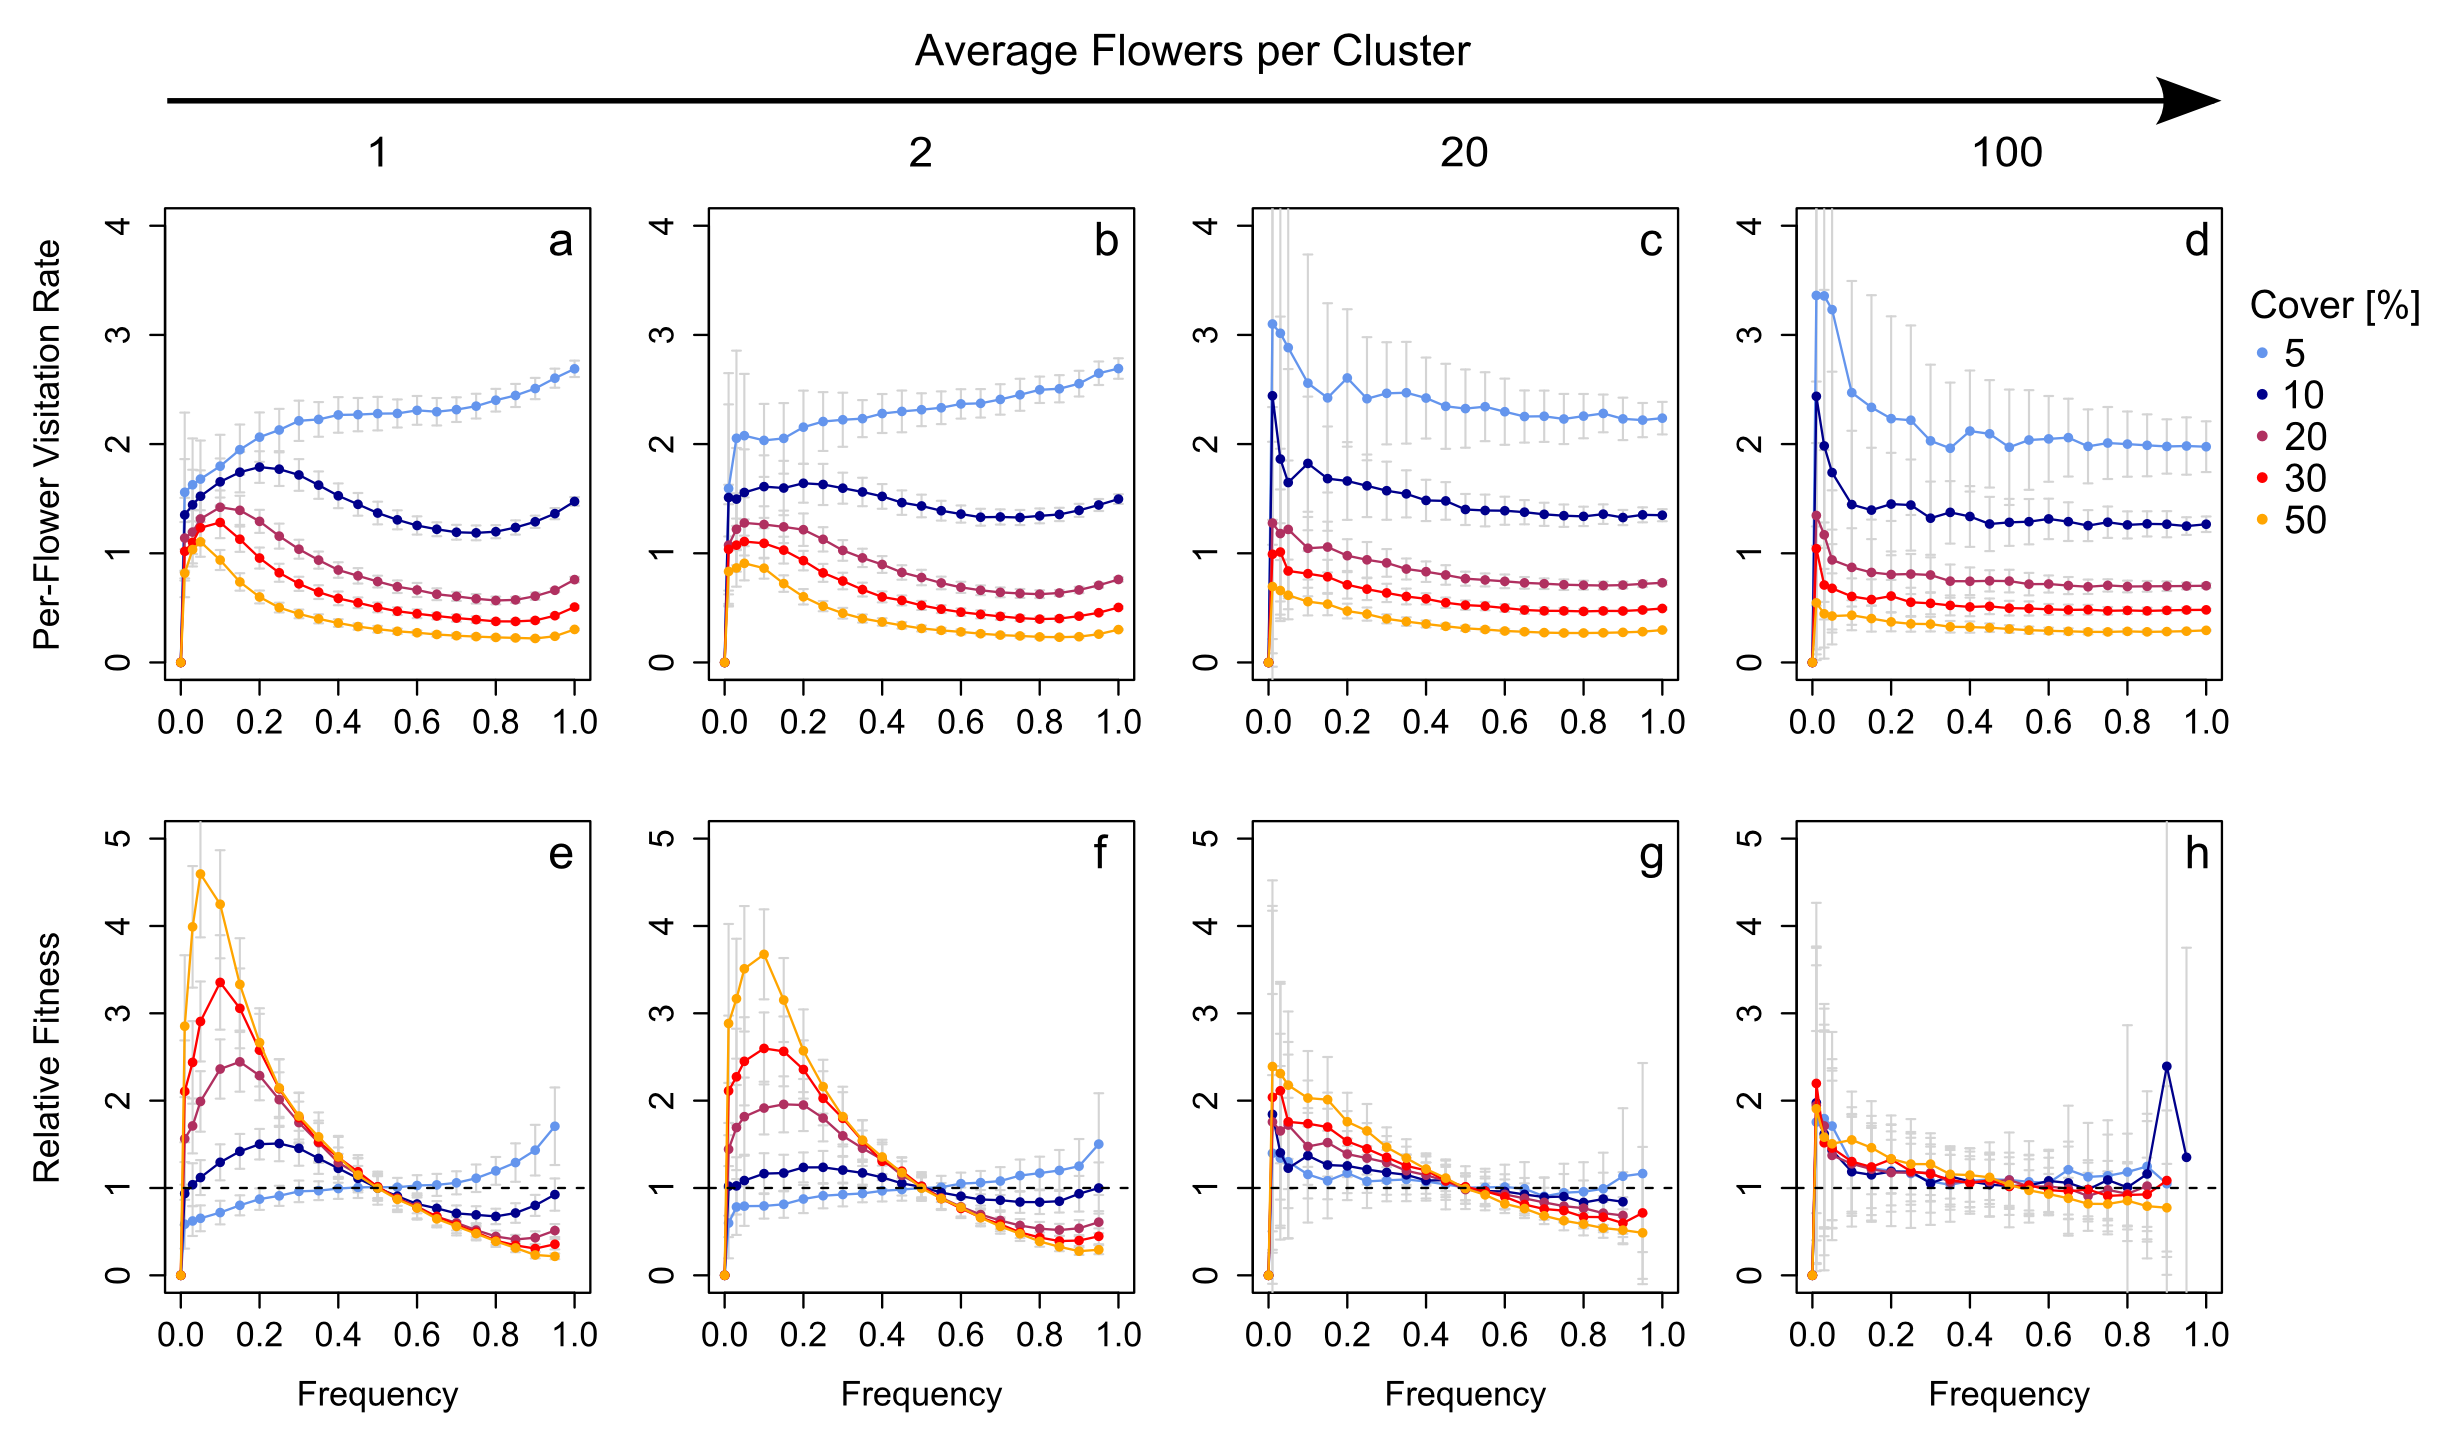
\includegraphics[width=17cm]{Images/PFV}
	\caption{The main analysis of the agent-based model confirm the findings of the linear mixed effect model of the field data: The per-flower visitation rate shows a clear frequency dependence with a cubic relationship. Visitation rates increase within the first 10-20\% of frequency towards a maximum. For intermediate frequencies is the increase of flowers not proportional with additional visits. The per-flower visitation rate only increases again towards exclusiveness of the species. The effect is stronger for higher floral cover (2a-d). Increase in clustering reduces the frequency dependence (1d,2d).}
	\label{fig:PFV}
\end{figure}


\begin{figure} [!ht]
	\centering
	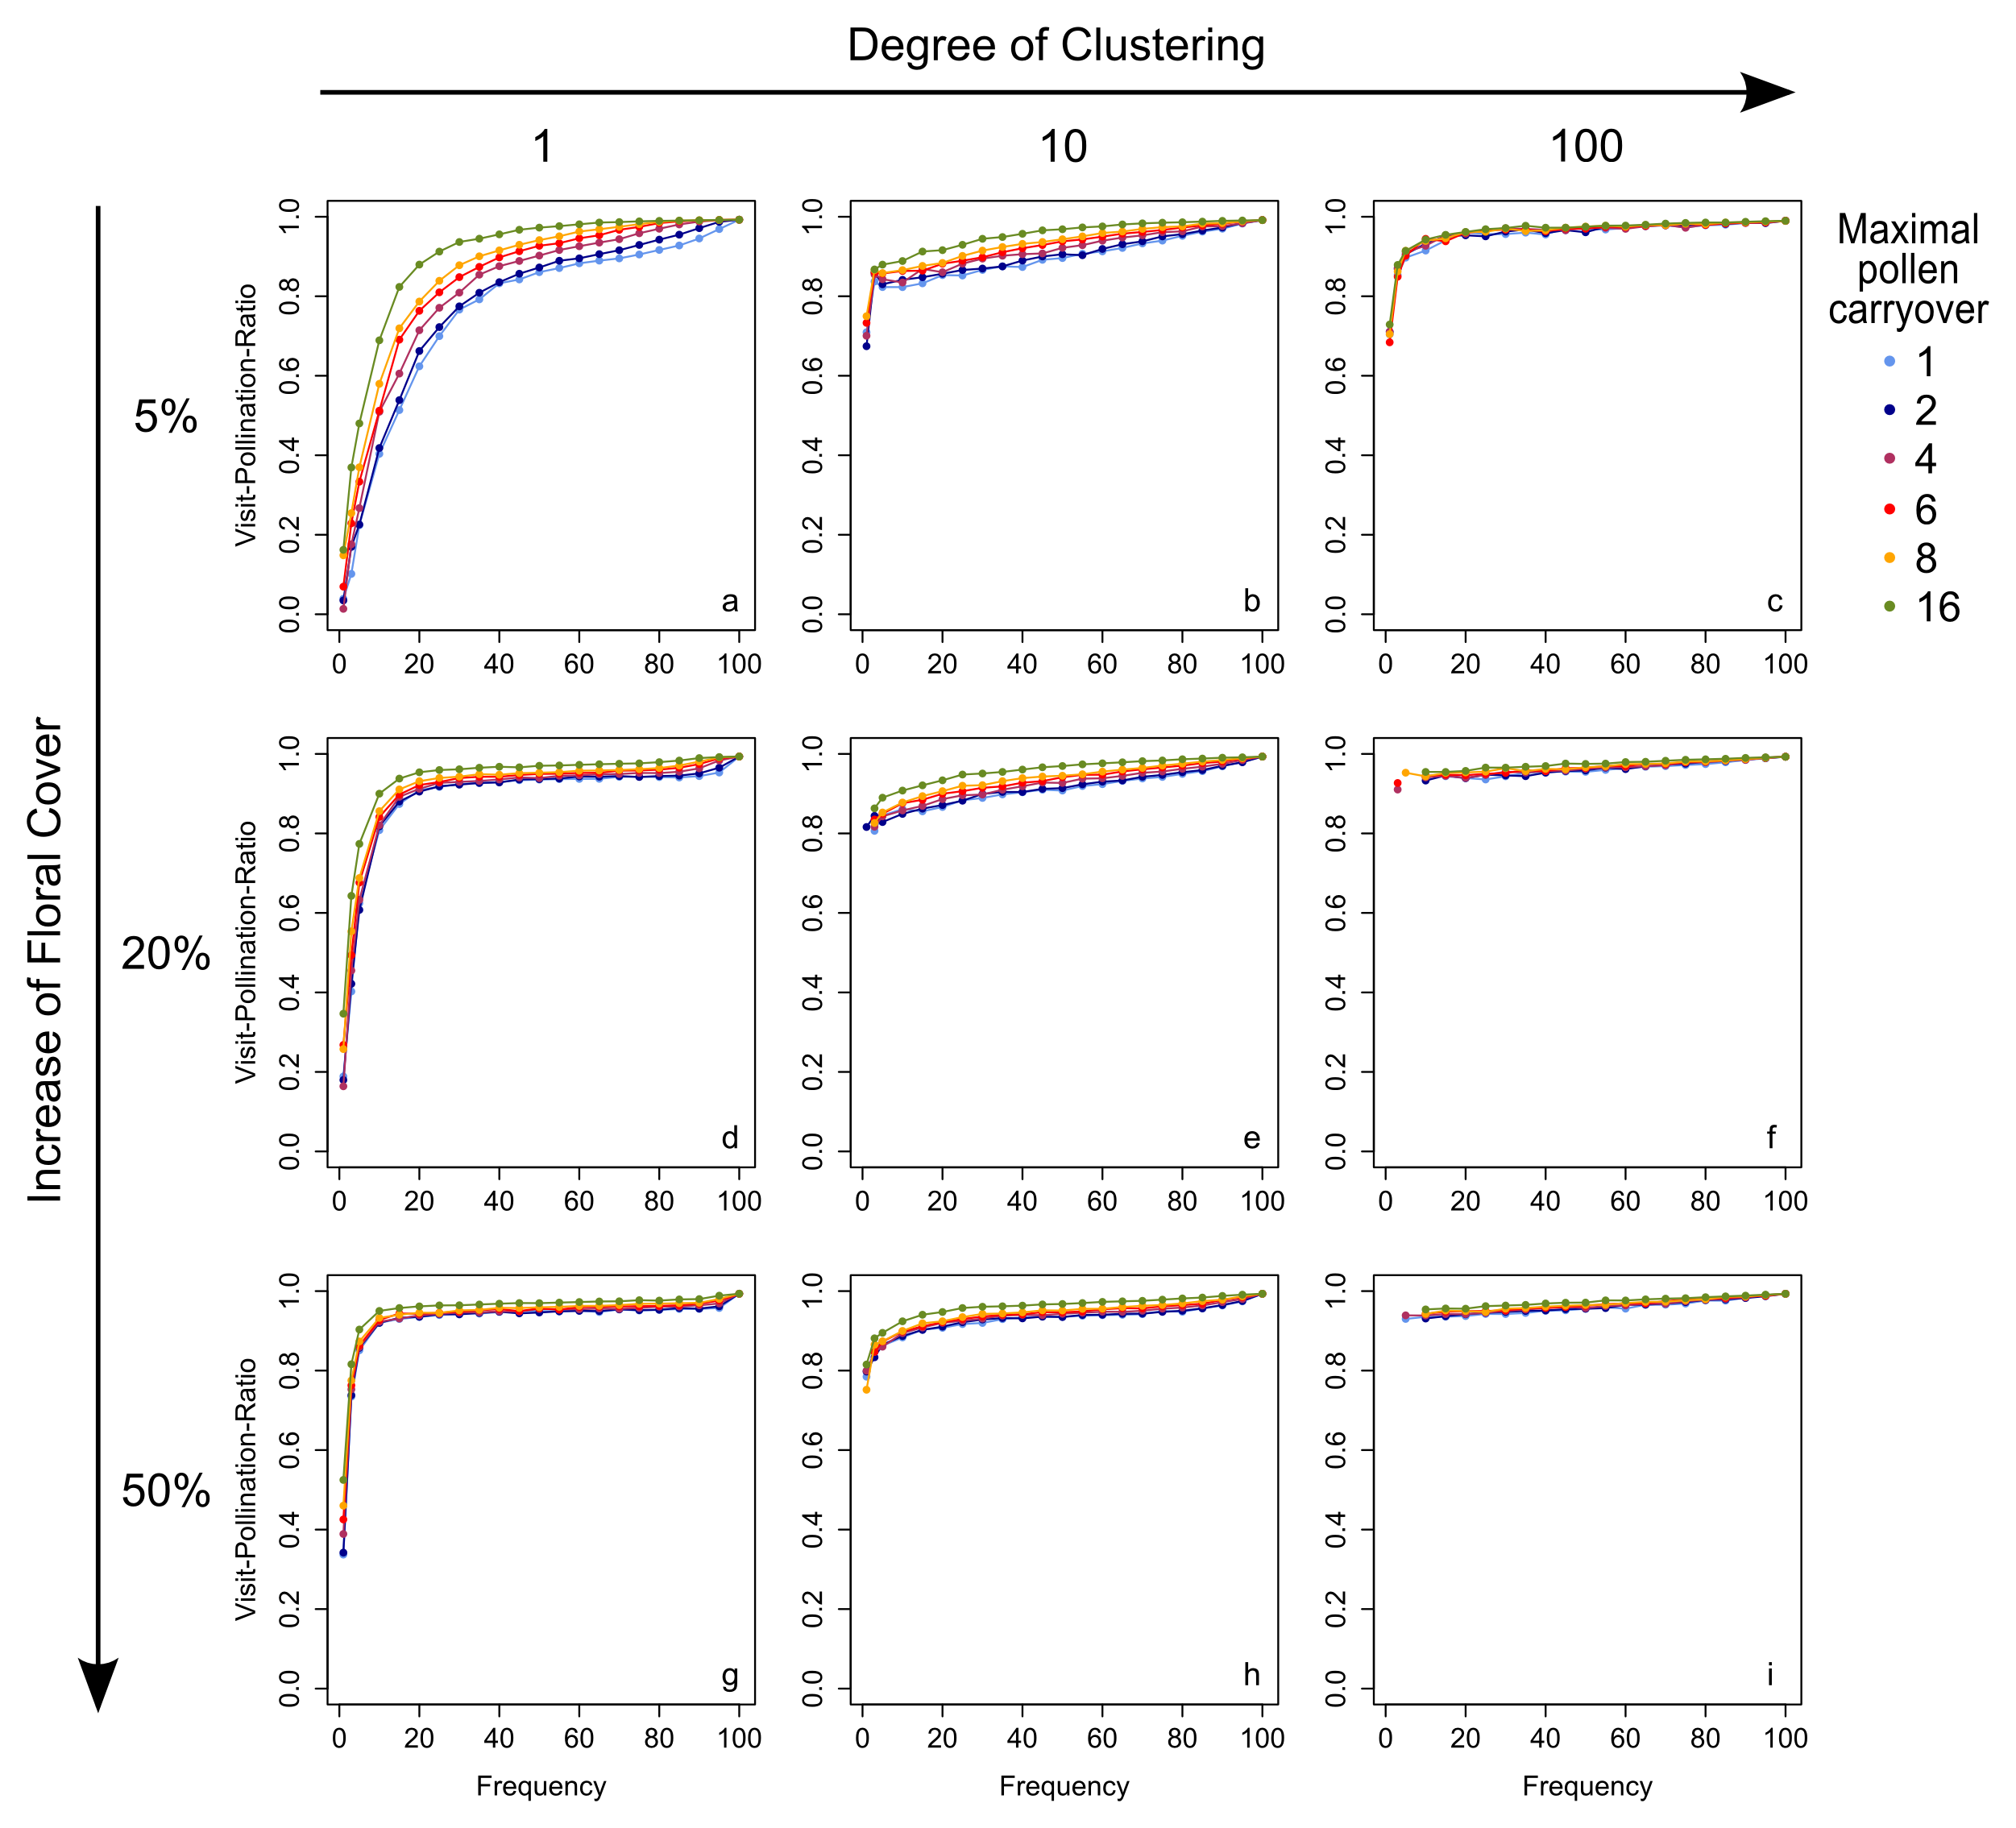
\includegraphics[width=17cm]{Images/POC}
	\caption{The pollen-carryover rate defines the maximum number of visits within a successful pollination is possible. With a pollen-carryover rate of one, the pollen can only be carried to the next flower. Therefore, the ratio of successful pollinations per visit can be seen as indicator for flower constancy \citep{montgomery2009pollen}. A high pollen-carryover rate is only important for a low cover and no-cluster environment. With increasing cover and cluster, the ratio becomes steeper for low frequencies which stands for more qualitative visits.}
	\label{fig:POC}
\end{figure}